tikz
\documentclass{standalone}
\usepackage{tikz}

\begin{document}
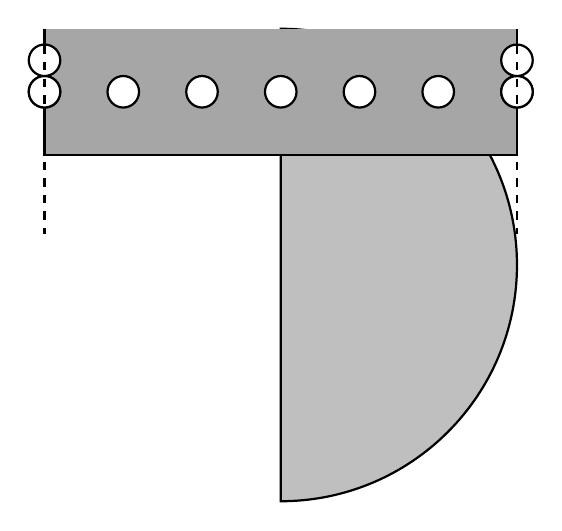
\begin{tikzpicture}[scale=2]

% Define the arch parameters
\def\archRadius{1.5} % Radius of the arch
\def\archHeight{0.8} % Height of the arch
\def\archWidth{3}    % Width of the arch

% Draw the arch
\draw[thick, fill=gray!50] 
  (0,\archHeight) arc (90:-90:\archRadius) -- cycle;

% Draw the bridge structure
\draw[thick, fill=gray!70]
  (-\archWidth/2, \archHeight) -- 
  (-\archWidth/2, 0) -- 
  (\archWidth/2, 0) -- 
  (\archWidth/2, \archHeight);

% Add some decorative elements
\foreach \x in {-1.5,-1,...,1.5}
  \draw[thick, fill=white] 
    (\x, \archHeight/2) circle (0.1);
\foreach \y in {0.4,0.6}
  \draw[thick, fill=white] 
    (-1.5, \y) circle (0.1);
\foreach \y in {0.4,0.6}
  \draw[thick, fill=white] 
    (1.5, \y) circle (0.1);

% Add some lines for support
\draw[thick, dashed]
  (-\archWidth/2, \archHeight) -- 
  (-\archWidth/2, -0.5);
\draw[thick, dashed]
  (\archWidth/2, \archHeight) -- 
  (\archWidth/2, -0.5);

\end{tikzpicture}
\end{document}